For an arc $\beta$ belonging to a Burau pair $(\alpha, \beta)$, we denote by $\vec{w}_\beta$ the corresponding weights on $\mu$, $c(\beta)$ the number of crossings with $\alpha$, and $p_\beta(t)$ the resulting Burau polynomial. For each $k \in \N$, \emph{the arcs of level $2k$} are $\set{\beta : c(\beta) = 2k}$. Our implementation has resulted in the following theorem.

\begin{theorem}
 For any arc $\beta$ with $c(\beta) \leq 2000$, $p_\beta(t) \neq 0$.
\end{theorem}

Finding no arc-pair asserting the unfaithfulness of $\Psi_4$, we proceed with a more qualitative analysis. Define the minimum norm and multiplicity of a level $2k$ to be
\begin{align*}
 \minnorm(2k) &= \min_{\beta} \set{|p_\beta(t)| : c(\beta) = 2k}\\
 \mult(2k) &= \#\set{\beta : |p_\beta(t)| = \minnorm(2k)}.
\end{align*}
The initial levels have erratic behavior.
\begin{center}
 \begin{tabular}{c|c|ccc|c|ccc|c|c}
  $2k$ & $\minnorm(2k)$ & $\mult(2k)$ & \  & $2k$ & $\minnorm(2k)$ & $\mult(2k)$ & \  & $2k$ & $\minnorm(2k)$ & $\mult(2k)$\\
  \cline{1-3} \cline{5-7} \cline{9-11}
  2 & 2 & 5 && 16 & 8 & 24 && 30 & 8 & 6\\
  4 & 4 & 37 && 18 & 8 & 6 && 32 & 8 & 12\\
  6 & 6 & 115 && 20 & 8 & 24 && 34 & 8 & 18\\
  8 & 6 & 20 && 22 & 6 & 6 && 36 & 10 & 36\\
  10 & 8 & 86 && 24 & 8 & 18 && 38 & 8 & 6\\
  12 & 8 & 30 && 26 & 8 & 12 && 40 & 8 & 18\\
  14 & 8 & 18 && 28 & 8 & 24 && 42 & 10 & 24\\
 \end{tabular}
\end{center}

However after this appears remarkable periodicity.
\begin{theorem}
 \label{thm:periodicity}
 For $2k \in [44, 500]$,
 $$
  \minnorm(2k) = \left\{\begin{array}{cc}10 & \text{if } 2k \equiv 0 \mod{6}\\ 8   & \text{otherwise} \end{array}\right. \qquad \mult(2k) = \left\{\begin{array}{cc}6 & \text{if } 2k \equiv 2 \mod{6}\\ 18 & \text{otherwise} \end{array}\right..
 $$
\end{theorem}
The periodic behavior in Theorem \ref{thm:periodicity} is a result of the arcs falling into into families. 
\begin{example}
 \label{exmample:minnormfamily}
 Let $2k \equiv 0 \mod{6}$ and $44 \leq 2k  \leq 500$. Setting $m = \frac{2k - 48}{6}$, the weights 
  $$w_0 = 22 + 2m,\ w_1 = 74 + 10m,\ w_2 = 89 + 12m,\ w_3 = 21 + 2m,\ w_{14} = 192 + 24m$$
 give rise to arcs $\set{\beta_m}_{m=0}^{158}$ with $c(\beta_m) = 2k$, $|p_{\beta_m}(t)| = \minnorm(2k)$, and
  $$p_{\beta_m}(t) = -t^{-5} - t^{-3} - t^{-2} - t^{0} - t^{18+3m} + t^{19+3m} - 2t^{20+3m} + t^{21+3m} - t^{22+3m}.$$
\end{example}

Our computations have shown that all arcs $\beta$ with $c(\beta) \in [44, 500]$ and $|p_\beta(t)| = \minnorm(c(\beta))$ fall into $6+18+18$ families whose weights are in an arithmetic progression and whose ordered set of coefficients of the resulting Burau polynomials are constant.

There are a variety of ways that these families arise, the simplest is as follows. Let $\beta$ be an arc, $p$ a point on $\beta$, and $\gamma$ a loop that only intersects itself or $\beta$ at $p$. Then with some perturbations one can construct new arcs by repeatedly inserting $\gamma$ into $\beta$. An example of this form is seen in Figure \ref{fig:exampleSimpleFamily}. Note that doing this does not guarantee that the resulting Burau polynomial norms will all be equal, nor that the resulting polynomials themselves will all be of a similar form. More complicated patterns also give rise to families, as seen in Figure \ref{fig:exampleComplexFamily} where there are two loops inserted in an interleaving fashion.

\begin{figure}[!h]
 \centering
 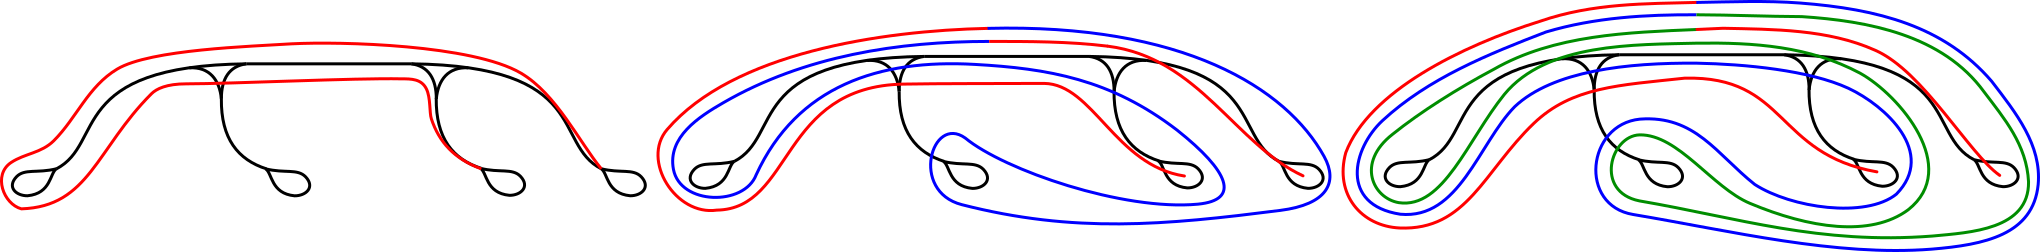
\includegraphics[width=.95\linewidth]{Family-simple.png}
 \captionof{figure}{Simple family of arcs.}
 \label{fig:exampleSimpleFamily}
\end{figure}

\begin{figure}[!h]
 \centering
 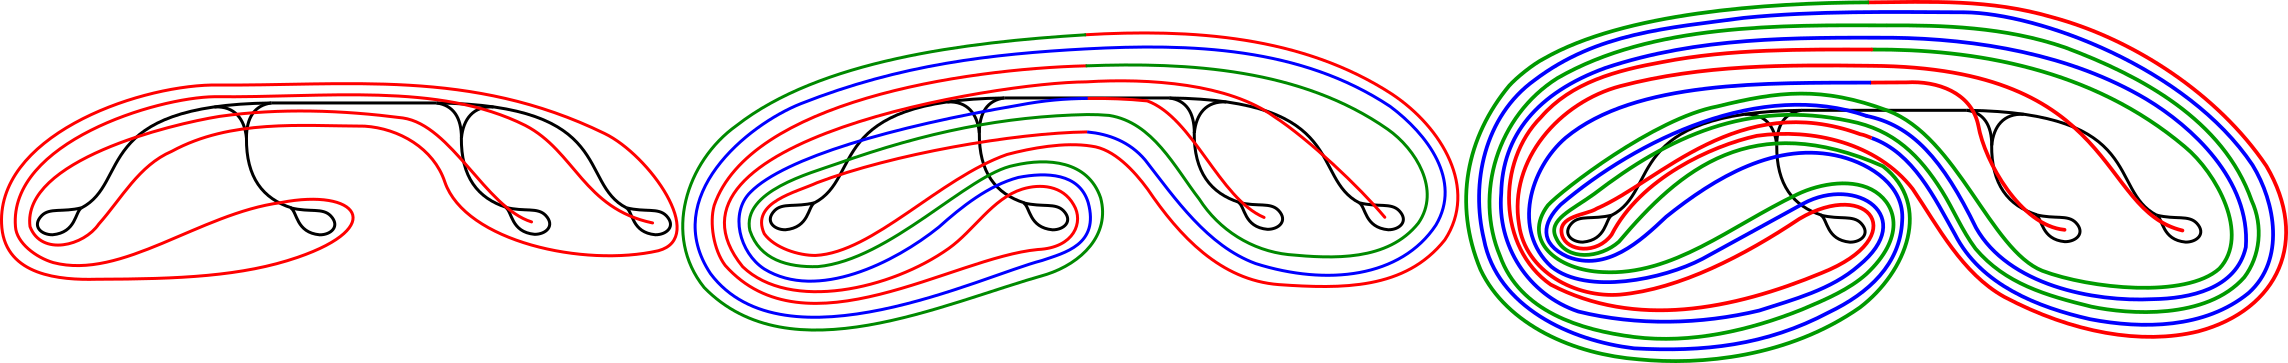
\includegraphics[width=.95\linewidth]{Family-complex.png}
 \captionof{figure}{Complex family of arcs.}
 \label{fig:exampleComplexFamily}
\end{figure}

The families in Figure \ref{fig:exampleSimpleFamily} and Figure \ref{fig:exampleComplexFamily} are not one of the $6+18+18$ families in Theorem \ref{thm:periodicity}. Indeed, the families in Theorem \ref{thm:periodicity} would be quite difficult to draw. In order to see their behavior, we can look at records of the arcs. Consider Example \ref{exmample:minnormfamily} above, but now with $m = \frac{2k - 6}{6}$ where $2k \equiv 0 \mod{6}$ and $2k \in [6, 500]$. The records of the first three members of this family are as follows.
 $$(3, 5, 3, 5, 4, 2, 4, 2, 4, 2, 4)$$
 $$\left(3, 5, 3, 5, \fbox{4, 1, 2, 4, 2, 4, 2, 5, 3, 5, 3, 5}, 4, 2, 4, 2, 4, 2, 4\right)$$
 $$\left(3, 5, 3, 5, \fbox{4, 1, 2, 4, 2, 4, 2, 5, 3, 5, 3, 5}, \fbox{4, 1, 2, 4, 2, 4, 2, 5, 3, 5, 3, 5}, 4, 2, 4, 2, 4, 2, 4\right)$$
The $m$th member is achieved by inserting the arc with record $4, 1, 2, 4, 
2, 4, 2, 5, 3, 5, 3, 5$ $m$-times. Another family of arcs that gives rise to the minimum norms of Theorem \ref{thm:periodicity} has the following records.
 $$(3, 5, 3, 5, 3, 5, 4, 2, 4, 2, 4)$$
 $$\left(\fbox{3, 5, 3, 5, 3}, \fbox{6, 5, 4, 2, 4, 2, 4}, 3, 5, 3, 5, 3, 5, 4, 2, 4, 2, 4\right)$$
 $$\left(\fbox{3, 5, 3, 5, 3}, \fbox{6, 5, 4, 2, 4, 2, 4}, \fbox{3, 5, 3, 5, 3}, \fbox{6, 5, 4, 2, 4, 2, 4}, 3, 5, 3, 5, 3, 5, 4, 2, 4, 2, 4\right)$$
Here the arcs $3, 5, 3, 5, 3$ and $6, 5, 4, 2, 4, 2, 4$ are interleaved. In each of these examples, the initial members of the family do not give rise to Burau polynomials with the same ordered set of coefficients. It is only the later members that have this behavior.

\/*\begin{center}
 \includegraphics[scale=0.25]{Family-simple01.png}
 \includegraphics[scale=0.25]{Family-simple02.png}
 \includegraphics[scale=0.25]{Family-simple03.png}
\end{center}


More complicated patterns also arise.

\begin{center}
 \includegraphics[scale=0.3]{Family-complex01.png}
 \includegraphics[scale=0.3]{Family-complex02.png}
 \includegraphics[scale=0.3]{Family-complex03.png}
\end{center}

In the family above, each additional step inserts two loops; one blue and one green.  Due to the way they are interleaved, the number of blue loops must equal that of green loops. 

While neither of these two families give rise to arcs that achieve minimum norm, the behavior of those that do is similar. We can see this by looking at the logs of the arcs. The first family pictured above has the following logs.
 $$(4)$$
 $$(4, 1, 2, 5, 4)$$
 $$(4, 1, 2, 5, 4, 1, 2, 5, 4)$$
 $$(4, 1, 2, 5, 4, 1, 2, 5, 4, 1, 2, 5, 4)$$
The insertion of the blue loop can be seen by the insertion of $1, 2, 5, 4$ in the log. The second family pictured above has the following logs.
 $$(5, 6, 7)$$
 $$(6, 1, 5, 6, 7, 6, 7)$$
 $$(6, 1, 6, 1, 5, 6, 7, 6, 7, 6, 7)$$
 $$(6, 1, 6, 1, 6, 1, 5, 6, 7, 6, 7, 6, 7, 6, 7)$$
The red arc is $5, 6, 7$, the blue arc is $6, 1$, and the green arc is $6, 7$.

The same behavior occurs in all of the minimum norm weights mentioned above. For example, consider the family ${8 + 2k, 4 + 10k, 5 + 12k, 7 + 2k, 24 + 24k}$ where we now set $k = \frac{c - 6}{6}$ with $c \equiv 0 \mod{6}$ and $c \in [6, 500]$. This is the family of minimum norm discussed above. The logs of the first three members of this family are as follows.
 $$(3, 5, 3, 5, 4, 2, 4, 2, 4, 2, 4)$$
 $$(3, 5, 3, 5, 4, 1, 2, 4, 2, 4, 2, 5, 3, 5, 3, 5, 4, 2, 4, 2, 4, 2, 4)$$
 $$(3, 5, 3, 5, 4, 1, 2, 4, 2, 4, 2, 5, 3, 5, 3, 5, 4, 1, 2, 4, 2, 4, 2, 5, 3, 
5, 3, 5, 4, 2, 4, 2, 4, 2, 4)$$
In this family, the $k$th member is achieved by inserting the arc $4, 1, 2, 4, 
2, 4, 2, 5, 3, 5, 3, 5$ $k$-times. The 
families of minimum norm also exhibit more complex patterns. For example, the weights $(20, 76, 91, 19, 192)$ occurs in a family whose logs are as follows.
 $$(3, 5, 3, 5, 3, 5, 4, 2, 4, 2, 4)$$
 $$(3, 5, 3, 5, 3, 6, 5, 4, 2, 4, 2, 4, 3, 5, 3, 5, 3, 5, 4, 2, 4, 2, 4)$$
 $$(3, 5, 3, 5, 3, 6, 5, 4, 2, 4, 2, 4, 3, 5, 3, 5, 3, 6, 5, 4, 2, 4, 2, 4, 3, 
5, 3, 5, 3, 5, 4, 2, 4, 2, 4)$$
Here the arcs $3, 5, 3, 5, 3$ and $6, 5, 4, 2, 4, 2, 4$ are interleaved.*/

Grouping the arcs into families, the periodicity observed in Theorem \ref{thm:periodicity} is recast into an observation about $6+18+18$ families. These families always being of minimal norm block us from seeing the behavior of other arcs. In order to see through this obstruction, we group all arcs into ``tightly-knit'' families and study the minimum norm where we ignore any noninitial member of such a family.

Let $\sF = \set{\beta_i}_{i=0}^\infty$ be a collection of arcs and set $\vec{d} = \vec{w}_{\beta_1} - \vec{w}_{\beta_0}$. We say that $\sF$ is a \emph{tightly-knit family} if for all $i \in \N$, $\vec{w}_{\beta_i} = \vec{w}_{\beta_0} + i \cdot \vec{d}$ and $p_{\beta_i}(t)$ has the same ordered set of coefficients as $p_{\beta_0}(t)$. We call this the \emph{tightly-knit family generated by $\beta_0$ and $\beta_1$}. For such a family we define $c(\sF) = c(\beta_0)$.

Note that any given arc can lie in many tightly-knit families. Let $\beta$ and $\beta'$ be two distinct arcs with the entries of $\vec{w}_{\beta'} - \vec{w}_{\beta}$ all nonnegative. Then $\beta$ and $\beta'$ lie in a tightly-knit family if and only if $\beta_0 = \beta$ and $\beta_1 = \beta'$ themselves generate a tightly-knit family. To check that $\beta$ and $\beta'$ belong to the same family in computations, we must restrict ourselves to testing the first $m \in \N$ members generated by $\beta$ and $\beta'$. In the results below, we first used $m=100$ and then $m=1000$. In each case, the results remain unchanged.

For $k \in \N$ we define 
 $$\min(2k) = \min_\beta \set{|p_\beta(t)| : c(\beta) = 2k \text{ and } \beta \notin \sF \text{ for any } \sF \text{ with } c(\sF) < 2k}.$$
Note that there exists a positive $k \in \N$ such that $\min(2k) = 0$ if and only if $\Psi_4$ is unfaithful. We emphasize that in computing $\min(2k)$ for $2k \in [2, 200]$, seen in Figure \ref{fig:tightlyKnitFamilies}, we only test the first $100$, and then $1000$, members to determine if a collection forms a tightly-knit family.

\/*\begin{figure}[!h]
  \centering
  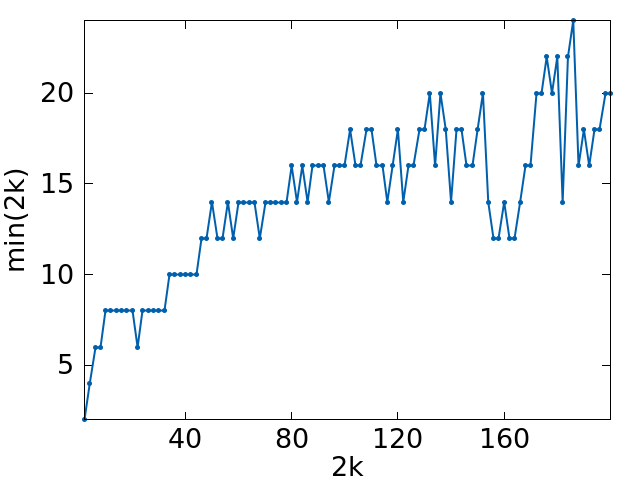
\includegraphics[width=6cm]{SmartEqualCoeffCap200.png}
  \captionof{figure}{Tightly-knit families}
  \label{fig:tightlyKnitFamilies}
\end{figure}*/

By weakening the definition of a tightly-knit family while maintaining the property that there exists a positive $k \in \N$ such that $\min(2k) = 0$ if and only if $\Psi_4$ is unfaithful, we can seek different ways to group the arcs into families, studying their behavior as the number of intersections increase. With this in mind, we say that $\sF = \set{\beta_i}_{i=0}^\infty$ is a \emph{loosely-knit} family if for all $i \in \N$, $\vec{w}_{\beta_i} = \vec{w}_{\beta_0} + i \cdot (\vec{w}_{\beta_1} - \vec{w}_{\beta_0})$ and $|p_{\beta_i}(t)| \geq |p_{\beta_0}(t)|$ for all $i \in \N$. The result of computing $\min(2k)$ for $2k \in [2, 200]$ using loosely-knit families is seen in Figure \ref{fig:looselyKnitFamilies}, again with the computational limitations as mentioned above.

\/*\begin{figure}[!h]
  \centering
  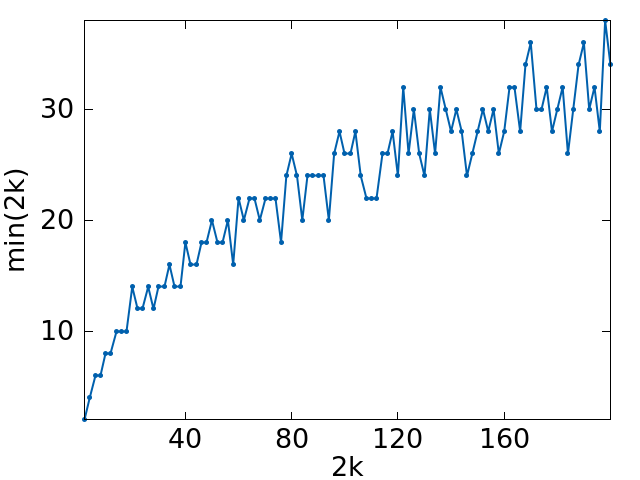
\includegraphics[width=6cm]{SmartAtLeastNorm.png}
  \captionof{figure}{Loosely-knit families}
  \label{fig:looselyKnitFamilies}
\end{figure}*/

\begin{figure}[!h]
 \centering
 \begin{subfigure}[t]{0.4\textwidth}
  \centering
  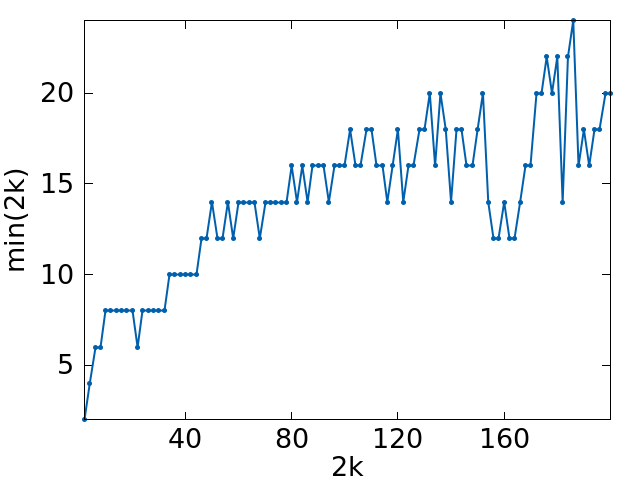
\includegraphics[width=2in]{SmartEqualCoeffCap200.png}  
  \caption{Tightly-knit families}
  \label{fig:tightlyKnitFamilies}
 \end{subfigure}
 \quad
 \begin{subfigure}[t]{0.4\textwidth}
  \centering
  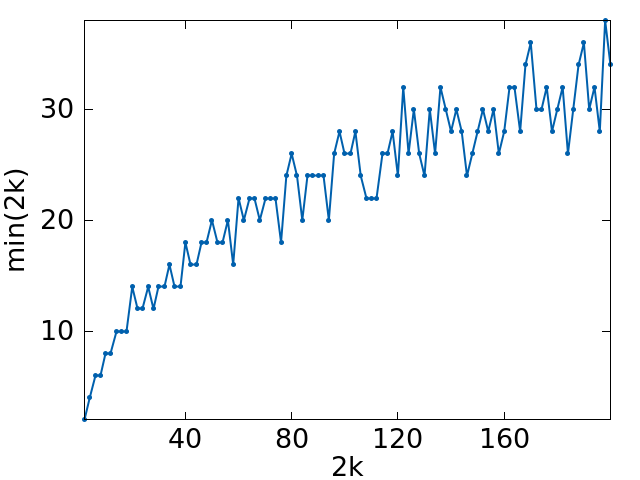
\includegraphics[width=2in]{SmartAtLeastNorm.png} 
  \captionof{figure}{Loosely-knit families}
  \label{fig:looselyKnitFamilies}
 \end{subfigure}
 \caption{}
\end{figure}

We interpret the upward trend of these graphs as being suggestive that $\Psi_4$ is faithful.